\chapter{Implementation}
In order to achieve the project objective, it was necessary for the Android application to establish communication with ATOS. An illustrative chart showcasing the integration process is presented below:

\begin{figure}[H]
  \centering
  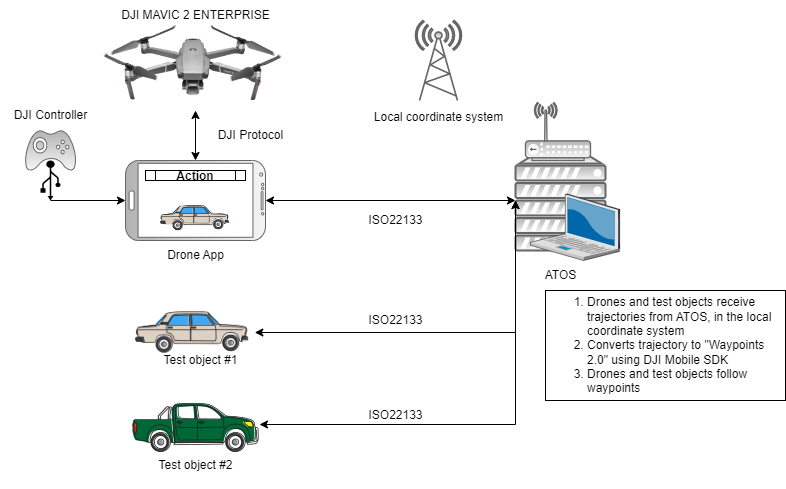
\includegraphics[width=\columnwidth]{figure/flow_config.png}
  \caption{Integration}
  \label{fig:ATOS-APP}
\end{figure}
The object-control module within the ATOS software facilitates the transmission of trajectories for drones and test-objects in the local coordinate system, situated on the AstaZero test track through the ISO22133 protocol. The drone application subsequently converts this data into global latitude and longitude coordinates, referred to as "Waypoints "\todo{ändrade detta då vi inte använder WP2.0 //MS}, through the utilization of the DJI Mobile SDK. Consequently, the drone application transmits the way-points to the drone by means of the DJI protocol, effectively initializing it. Following this, the test commences, and the drones and test objects following their pre-determined trajectories.

\section{Capabilities of existing software}

\subsection{Waypoint 1 Activity}
\subsection{Douglas-Peucker A}

\section{Implementation of missions}
\todo{Hitta nytt namn}

\section{Alternative to Douglas-Puecker algorithm}

\section{Implementation of image recognition}
\todo{Hitta nytt namn}

\section{Implementation of object tracking}
\todo{Hitta nytt namn}

\section{Integration and configuration}





% \subsection{Merging the apps}
% When both apps worked decently we tried merging the apps. Pretty quickly we realized the DJI SDK did not support running parallel missions in our case the waypoint mission and the activetrack mission. We are currently working on fixing this, by using the waypoint mission and running a convolutional neural network to identify cars on images from the video feed then using the pixel-coordinates of the object to adjust the gimbal.

